\subsection{Architecture Overview}
Our system is composed by two main component:
\begin{itemize}
    \item \textbf{server-side components:} the components include Identity and Access Management (\textbf{Keycloak}), database (\textbf{Postgres}), logic handler (\textbf{OpenABE}), MCP server.
    \item \textbf{client-side connectors:} adapter and hook grant connection and control over the AI agent.
\end{itemize}
The server-side components are designed to be each one indipendent from the others; we have containerized each one of them with \code{containerd} and made them available with Rancher Desktop.

Client-side there are two parts essential to the correct flow of the program: there is an adapter for each agent and a hook that is the real intermediary between the server-side and the agent.
\subsection{Early Prototyping: File Viewer and .abe format}

\subsubsection{File Structure} \label{File Structure}
To start approaching the concept, it is imperative to subdivide the problem into smaller ones. The first problem that came to mind was to find a way to have into a single file multiple parts, each with its own encryption.
To solve this problem, we did create a JSON structure that could contain each encrypted section of the file, i.e. an array containing a single object per section that has two properties: the policy requested to decipher the ciphertext and the ciphertext itself.
\begin{lstlisting}[language=JSON, caption={.abe format v1}]
{
  "format": "abe-doc",
  "version": 1,
  "sections": [
    {
      "policy": "livello = x",
      "chiphertext": CIPHERTEXT_Lx
    },
    {
      "policy": "livello = y",
      "chiphertext": CIPHERTEXT_Ly
    },
    {
      "policy": "livello = z",
      "chiphertext": CIPHERTEXT_Lz
    }
  ]
}
\end{lstlisting}
It's quite easy to point out that this implementation is very inefficient when the number of sections grows. To optimize the amount of operations needed and the structure of the document itself, it was improved in the version 2 of the structure:
\begin{lstlisting}[language=JSON, caption={.abe v2}]
{
  "format": "abe-doc",
  "version": 1,
  "sections": [
    {
      "group": 0
    },
    {
      "group": 1
    },
    {
      "group": 2
    },
    {
      "group": 1
    },
    {
      "group": 0
    }
  ],
  "groups": [
    {
      "policy": "livello >= 3",
      "ciphertext": CIPHERTEXT_L3
    },
    {
      "policy": "livello >= 2",
      "ciphertext": CIPHERTEXT_L2
    },
    {
      "policy": "livello >= 1",
      "ciphertext": CIPHERTEXT_L1
    }
  ]
}
\end{lstlisting}
This structure provides one key feature: the ability to call the decrypt function $n$ times, where $n$ is the number of unique attributes used to rules the sections. This is a more sustainable approach than v1, since, in that case, the decrypt function would be called exactly $m$ times, where $m$ is the amount of each section in the document. It's a fair assumption to say that $m$, \textit{usually}, is greater than $n$.
\subsubsection{File Viewer}
Having a structured document by itself was not sufficient for our testing needs and, having the need to read and edit a \code{.abe} file, it was necessary to create such application. The file viewer operates as a simple file editor, with the ability to encrypt and decrypt a file using a user's private key (N.B. this feature would negate entirely the Keycloak IAM workflow and was created only for test).
% TODO: POSSIBLE EDIT NEEDED (Keycloak > stored key)
This private key, as seen before, 
% Reference a previous explaination of the ABE
has to be created and stored beforehand. A user could also authenticate itself via \textbf{Keycloak} login and so a token with its attribute will be elaborated and used in substitution of the user's key.
The user-intended workflow is to login with \textbf{Keycloak} and only then he'd have access to the decryption of sections to him destinated.

There is an implicit security system, that is any user with the "security level" (an attribute defined to test a hierarchy) less than the maximum security level used in the file cannot overwrite the file.
\subsection{CP-ABE Authority and Key Management}
It is clear that we have to have a central autorithy that could audit and grant accesses to documents. This operation is made by conjuncting both \textbf{Keycloak} and \textbf{Postgres}:
While \textbf{Keycloak} holds every user's informations (e.g. mail, department, security level, etc...), and so its attributes, \textbf{Postgres} holds both the users' cached keys, once they recieved them from Keycloak, and a list of allowed agents with each own key.

% TODO: Explain better this part
The concept is simple: first a user get its token from Keycloak, then a cached and hashed key is kept in memory in a trusted sql database, and then, if in said database is found a key corresponding to the user's agent, the request is accepted by the server who will run the \textbf{OpenABE} operations to serve the decrypted file.
With this solution nobody needs to have installed its own key and it is strictly handled "in background", to both minimizing the risk of tampering and also to ensure a strict control over the allowed agents (it's easy as deleting a row in a db to disable entirely an agent from being used).

\subsection{Human Identity via Keycloak}
Obviously, the Keycloak login can and has to be used with two-factor-authentication (it can be enforced also a biometric login). The 2fa itself is out of this scope, but we mention \textbf{FreeOTP} as a free tool for an otp testing.

Once the user is logged in, and we can assume it is authenticated, then we can proceed to concede a token, containing the relevant attributes, that will be used to ask for the key of said user.

\subsection{Agent Identity Model}

\subsection{Audit Logging}
Each and every operation the agent make while calling the server is logged, both to log every access to each document and to ensure their confidentiality.
Server-side it is all kept in a \code{audit.jsonl}, for semplicity's sake, but it can be enhanced.


\subsection{Core and Strategy Pattern}

\subsubsection{The Relay Hook}

\subsubsection{Per-Agent Adapters}
Since each agent has its own way to be controlled, it is necessary to create a specific adapter for each one of them. The adapter is the component that will translate the generic workflow into agent-specific ones.
The general approach is to fold the content of the decision into the agent's reasoning process, so that if the decision is \code{None}, or better, if there is a deny from the \code{core.decide} function, then the agent will not be able to access the document and so it will not be able to use it in its reasoning process.
This is important because each and every agent has its own way to reason and use hooks, for example, Claude code uses \code{decision.updated\_input}, thanks to which we can impose the use of our tool; different story is for Copilot CLI we cannot fully rely to \code{additionalContext}.

Following we can see fragments of those two implementations for Claude code and Copilot CLI, respectively:
\begin{lstlisting}[language=Python, caption={Claude code adapter}]
def render(decision: Decision) -> RenderedResponse:
    if decision.kind == DecisionKind.ALLOW:
        if decision.updated_input is None:
            return RenderedResponse()  # no output at all - the tool call proceeds untouched
        # A direct call to pabel's own tools, allowed through with this
        # installation's agent credential injected - see core/decide.py.
        return RenderedResponse(stdout=json.dumps({
            "hookSpecificOutput": {
                "hookEventName": "PreToolUse",
                "permissionDecision": "allow",
                "updatedInput": decision.updated_input,
            }
        }))

    output = {
        "hookSpecificOutput": {
            "hookEventName": "PreToolUse",
            "permissionDecision": "deny",
            "permissionDecisionReason": decision.reason,
        }
    }
    if decision.content is not None:
        output["hookSpecificOutput"]["additionalContext"] = json.dumps(decision.content)
    return RenderedResponse(stdout=json.dumps(output))
\end{lstlisting}
\begin{lstlisting}[language=Python, caption={Copilot CLI adapter}]
def render(decision: Decision) -> RenderedResponse:
    if decision.kind == DecisionKind.ALLOW:
        return RenderedResponse()

    # The guaranteed channel: fold the relay result into the reason text
    # itself, since additionalContext delivery is unreliable here.
    reason = fold_content_into_reason(decision)
    output = {
        "hookSpecificOutput": {
            "hookEventName": "preToolUse",
            "permissionDecision": "deny",
            "permissionDecisionReason": reason,
        }
    }
    if decision.content is not None:
        output["hookSpecificOutput"]["additionalContext"] = json.dumps(decision.content)
    return RenderedResponse(stdout=json.dumps(output))
\end{lstlisting}
\subsection{Document Lifecycle}
The document starts its life whenever it is created and encrypted by somenoe, say a manager, that has to include sensible information in said document.
Once the appropriate policy is defined and used to encrypt the document, it is stored and it become available through requst at the MCP server.

\begin{figure}[h]
  \centering
  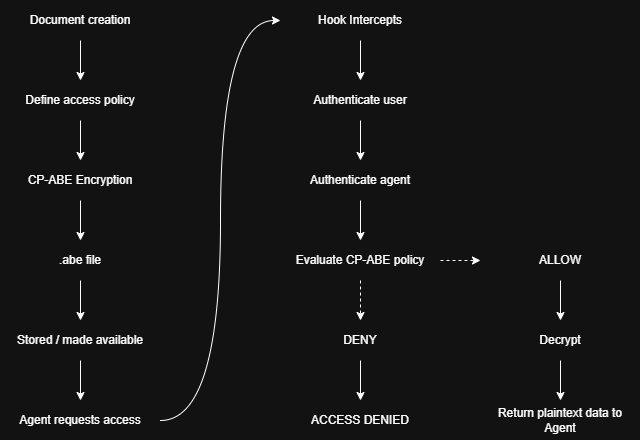
\includegraphics[width=\textwidth]{media/diagrams/Document Lifecycle.drawio.png}
  \caption{The flow diagram of the document lifecycle}
\end{figure}

When an agent requests access to a document, the hook will intercept the request and will start the authentication, first of the user and then of the agent. Everything is used to evaluate the CP-ABE policy and, if the user and the agent are both allowed to access the document, then the decryption will be performed and the document will be sent back to the agent; if not, the request will be denied and the agent will not have access to the document.


\subsection{Deployment Architecture}

